In this section, we choose two example queries (in Section \ref{S71} and \ref{S72}) from JOB as case study to obtain some insights into \textit{query split}. We demonstrate the detailed execution plan of \textit{query split} on these queries by Figure \ref{F15} and \ref{F16}, and explain what makes \textit{query split} faster than PostgreSQL, then discuss our findings from case studies in Section \ref{S73} and Section \ref{S74}.\par
Before analyzing the examples, we introduce the marks that will appear in the figures. In Figure \ref{F15} and \ref{F16}, the percentage next to the execution node represents the ratio of the time spent by the physical operator to the \textbf{total execution time} of \textit{query split}. The colored line represents the boundary of subqueries. The number above the relational algebra represents the estimated and actual size of intermediate results. As the estimation results at the subquery boundaries are precise, we just show the actual value.

\subsection{The First Case} \label{S71}
    \begin{figure}[htb]
        \subfigure[The join graph of example query 1]
        {
            \begin{minipage}[t]{0.9\linewidth}
                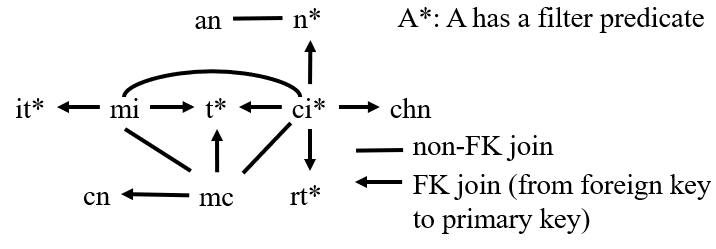
\includegraphics[width=\linewidth]{./pic/Figure15a.png}
            \end{minipage}
        }
        \subfigure[Execution plan of PostgreSQL]
        {
            \begin{minipage}[t]{0.47\linewidth}
                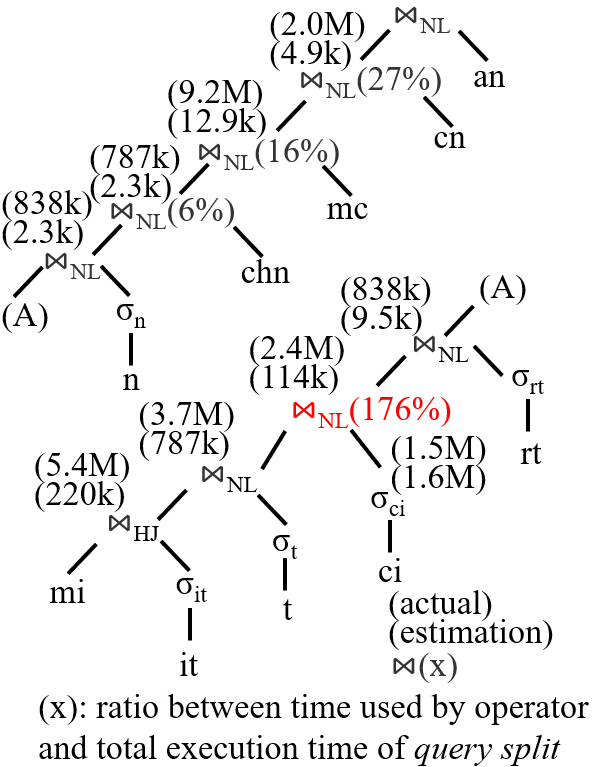
\includegraphics[width=\linewidth]{./pic/Figure15b.png}
            \end{minipage}
        }
        \subfigure[Execution plan of \textit{query split}]
        {
            \begin{minipage}[t]{0.47\linewidth}
                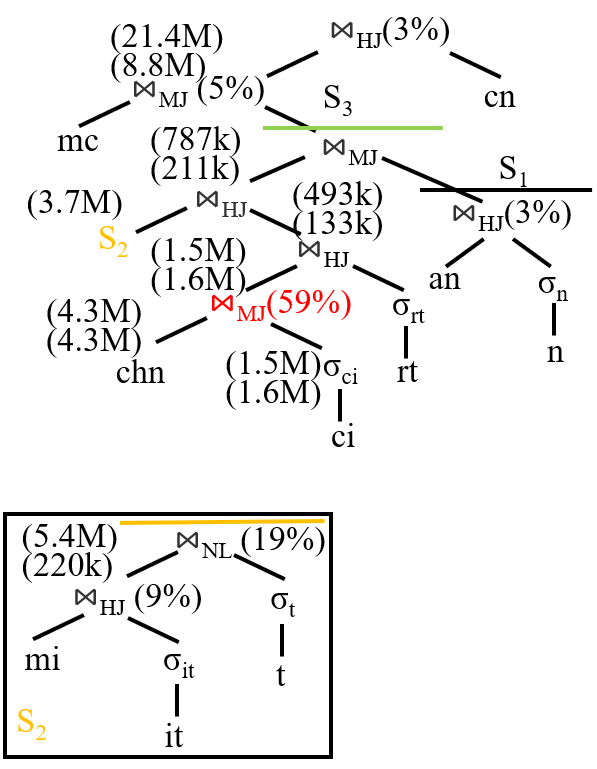
\includegraphics[width=\linewidth]{./pic/Figure15c.png}
            \end{minipage}
        }
        \centering
        \caption{The detail of query execution for example 1}
        \label{F15}
        \Description{}
    \end{figure}\par
    As shown in Figure \ref{F15}, there is a big gap between the cardinality estimation errors in PostgreSQL and query split. We use q-error \cite{paper53}, the factor by which the estimation differs from the true cardinality, to measure the quality of cardinality estimation. The average q-error in PostgreSQL is 246, while in \textit{query split} it is only 5.\par
    Another major difference in the execution plan between PostgreSQL and \textit{query split} is about how to deal with the join with table \textbf{ci}. In PostgreSQL, the execution plan directly join \textbf{ci} with the current intermediate result by nest loop. However, it's unwise because both left and right subtree are huge. As shown in Figure \ref{F15}(b), this nest loop costs too much time. In contrast, the decision of \textit{query split} is much better. As shown in Figure \ref{F15}(c), execution plan in \textit{query split} first decreases the size of table \textbf{ci} by joining with entity relations \textbf{chn} and \textbf{rt}. Note that although \textbf{chn} is huge as well, merge join can be applied without sorting and use much less time. Then, after the size of \textbf{ci} is reduced, it is joined with $S_2$. This decision effectively improves a time-consuming join in PostgreSQL and speeds up the query execution (from 128s to 48s).

\subsection{The Second Case} \label{S72}
    \begin{figure}[htb]
        \subfigure[The join graph of example query 2]
        {
            \begin{minipage}[t]{0.9\linewidth}
                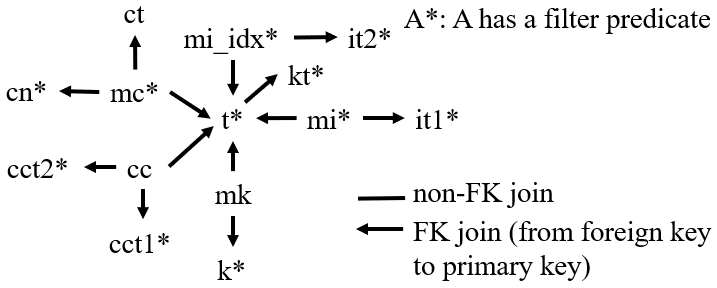
\includegraphics[width=\linewidth]{./pic/Figure16a.png}
            \end{minipage}
        }
        \subfigure[Execution plan of PostgreSQL]
        {
            \begin{minipage}[t]{0.47\linewidth}
                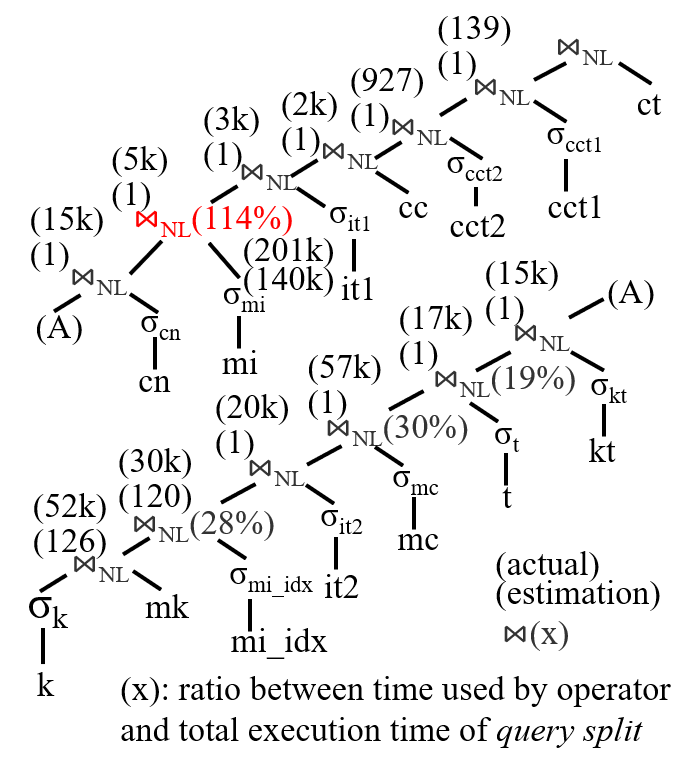
\includegraphics[width=\linewidth]{./pic/Figure16b.png}
            \end{minipage}
        }
        \subfigure[Execution plan of \textit{query split}]
        {
            \begin{minipage}[t]{0.47\linewidth}
                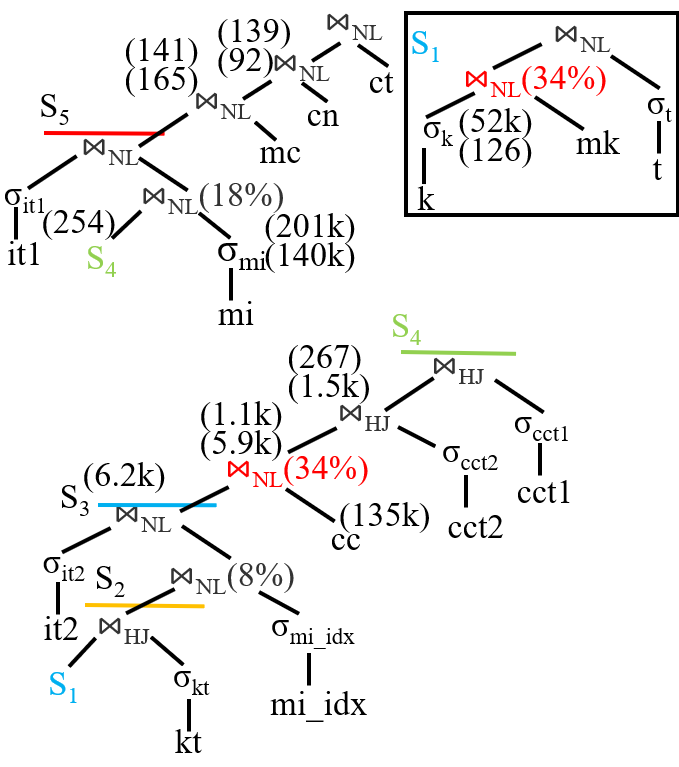
\includegraphics[width=\linewidth]{./pic/Figure16c.png}
            \end{minipage}
        }
        \centering
        \caption{The detail of query execution for example 2}
        \label{F16}
        \Description{}
    \end{figure}\par
    As shown in Figure \ref{F16}, there is also a big gap between the cardinality estimation errors in PostgreSQL and query split. The average q-error in PostgreSQL is 11310, while in \textit{query split} it is 37.\par
    Figure \ref{F16}(b) illustrates that the poor performance of PostgreSQL is due to using too much time to join table \textbf{mi}, where two huge inputs are involved. As shown in Figure \ref{F16}(c), in \textit{query split}, the optimizer postpones the join with \textbf{mi}, and instead decreases the size of inputs first. So when the join with \textbf{mi} happens in \textit{query split}, the size of another input is relatively small, which makes the execution faster.

\subsection{Our Findings} \label{S73}
    Now we can generalize two findings from case studies. First, the plan produced by \textit{query split} is close to \textit{optimal plan}. This is due to two reasons:
    \begin{itemize}[leftmargin = 15pt]
        \item The execution plan in each subquery is near-optimal. By gathering run-time statistics after the execution of each subquery, optimizer can get precise statistics of base relations in subqueries. Meanwhile, the size of each subquery is small. Under such conditions, cardinality estimation of the database optimizer is relatively accurate.
        \item By considering both result size and execution time, we can make a decent decision on subquery execution order. We postpone the execution of long-time join and decrease its size by replacing original inputs with other subqueries' results.
    \end{itemize}\par
    Second, we find that both queries are dominated by a very slow physical operator that consumes a massive piece of time (i.e. merge join and nest loop join), which takes more than half of the total execution time. We study this topic further in Section \ref{S74} to reveal remaining bottlenecks of query execution when the join order is good enough, and thus can help us further improve the query execution performance.

\subsection{A Further Study on Physical Operator} \label{S74}
    The phenomenon that the execution time is dominated by a single physical operator is in fact quite common in JOB. To study this topic further, we classify queries in JOB according to the operator that takes the longest time during execution, as shown in Table \ref{T5}.
    \begin{table}[htb]
        \caption{The physical operators that dominate JOB queries}
        \label{T5}
        \begin{tabular}{c|m{5cm}}
            \toprule
            physical operator & query Ids \\
            \hline
            hash join & 16, 23, 24, 28, 30, 55, 61, 81 \\
            \hline
            merge join & 46, 54 \\
            \hline
            index scan & 1, 2, 3, 4, 5, 6, 7, 8, 9, 10, 11, 12, 13, 15, 17, 19, 20, 21, 22, 29, 31, 32, 33, 34, 35, 36, 37, 38, 39, 40, 42, 45, 46, 47, 48, 49, 53, 56, 57, 62, 63, 64, 65, 66, 67,68, 69, 70, 71, 72, 73, 74, 75, 76, 77, 78, 79, 80, 82, 83, 84, 85, 86, 87, 88, 89, 90, 91 \\
            \hline
            sequential scan & 14, 18, 25, 26, 27, 41, 43, 44, 50, 51, 52, 58, 59, 60 \\
            \bottomrule
        \end{tabular}
    \end{table}\par
    We find that most queries are dominated by an index scan and other queries are dominated by hash join, merge join, or sequential scan.\footnote[4]{Note that our conclusion is derived from JOB, in which the number of queries is limited, and queries are human-write. The above reasons may cause our conclusion to be particular for JOB but not general for other benchmarks.} In the following part, we will discuss each of these operators.

    \subsubsection{Hash Join and Merge Join}
        It is possible further improve \textit{hash join} and \textit{merge join} by using a new and faster physical operator, \textit{directmap join}. In \textit{hash join}, to fetch an inner tuple, we need two random memory accesses: one for probing the hash table, another for accessing the inner tuple. If we reduce the number of memory accesses to once, we can achieve a faster execution speed.\par
        By combining probing and accessing data together, \textit{directmap join} can fetch a matching inner tuple through one memory access. Like \textit{hash join}, \textit{directmap join} consists of two phases: build phase and probing phase. In build phase, we copy the data of inner relation into a two-dimension array called \textit{map}, which can be treated as a combination of hash table and relation data. Due to the join attribute values in JOB being non-negative integer and having limited range, we simply use the original value as hash value ($hash(x)=x$), and each row of \textit{map} is used to store an inner tuple.
        \begin{figure}[htb]
            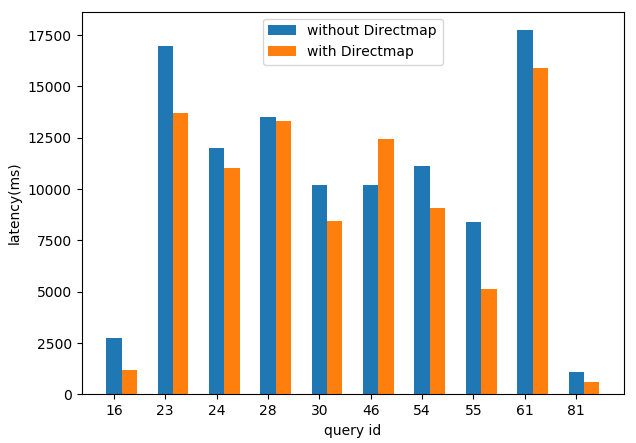
\includegraphics[width=\linewidth]{./pic/Figure17.png}
            \caption{The effect of \textit{directmap} on queries with join operator bottleneck}
            \label{F17}
            \Description{}
        \end{figure}\par
        In probe phase, for each tuple from outer relation with join attribute value $x$, we fetch the corresponding row $\textit{map}[x]$ and return the inner tuple if it is not empty. In this way, when probing and accessing an inner tuple, we only use one random memory access. We will explain the detailed implementation of \textit{directmap join} in Appendix \ref{A3}.\par
        We use \textit{directmap join} in those join operator constraint queries, and compare their execution time with previous results. The end-to-end latencies are shown in Figure \ref{F17}. Query 16, 55 and 81 have more than 50\% improvement in end-to-end latency, and query 23, 30 and 54 have nearly 25\% improvement. The result proves that \textit{directmap join} can greatly improve the total execution time for queries with join operator as bottleneck.
        

    \subsubsection{Index Scan and Sequential Scan}
        Unlike hash join and merge join, the queries dominated by \textit{index scan} and \textit{sequential scan} are hard to improve due to three reasons:
        \begin{enumerate}[leftmargin = 15pt]
            \renewcommand{\labelenumi}{\theenumi.}
            \item The use of scan operators is inevitable. 
            \item As far as we know, apart from \textit{index scan} and \textit{sequential scan}, there are no other comparable scan operators. In other words, if the optimizer has chosen the better scan operator between \textit{index scan} and \textit{sequential scan}, then there is little room for further improvement. 
            \item According to the cost model in PostgreSQL \cite{manual2}, we substitute the true cardinality into the cost model and find the scan operator decision made by the optimizer is indeed correct in \textit{query split}.
        \end{enumerate}\par
        From above three points, we conclude that there is no room to further improve \textit{index scan} and \textit{sequential scan} in \textit{query split}. Hence, under the dynamic query optimization framework, for most queries dominated by a scan operator, \textit{query split} is already a nearly optimal solution. Although there might exist some other strategies to further improve scan operators, such strategy are beyond the scope of our paper.